\section{Technical realization}\label{sect:realization}

\begin{figure*}[t]
	\centering
	\subfloat[Single Phase MPC Protocol]{{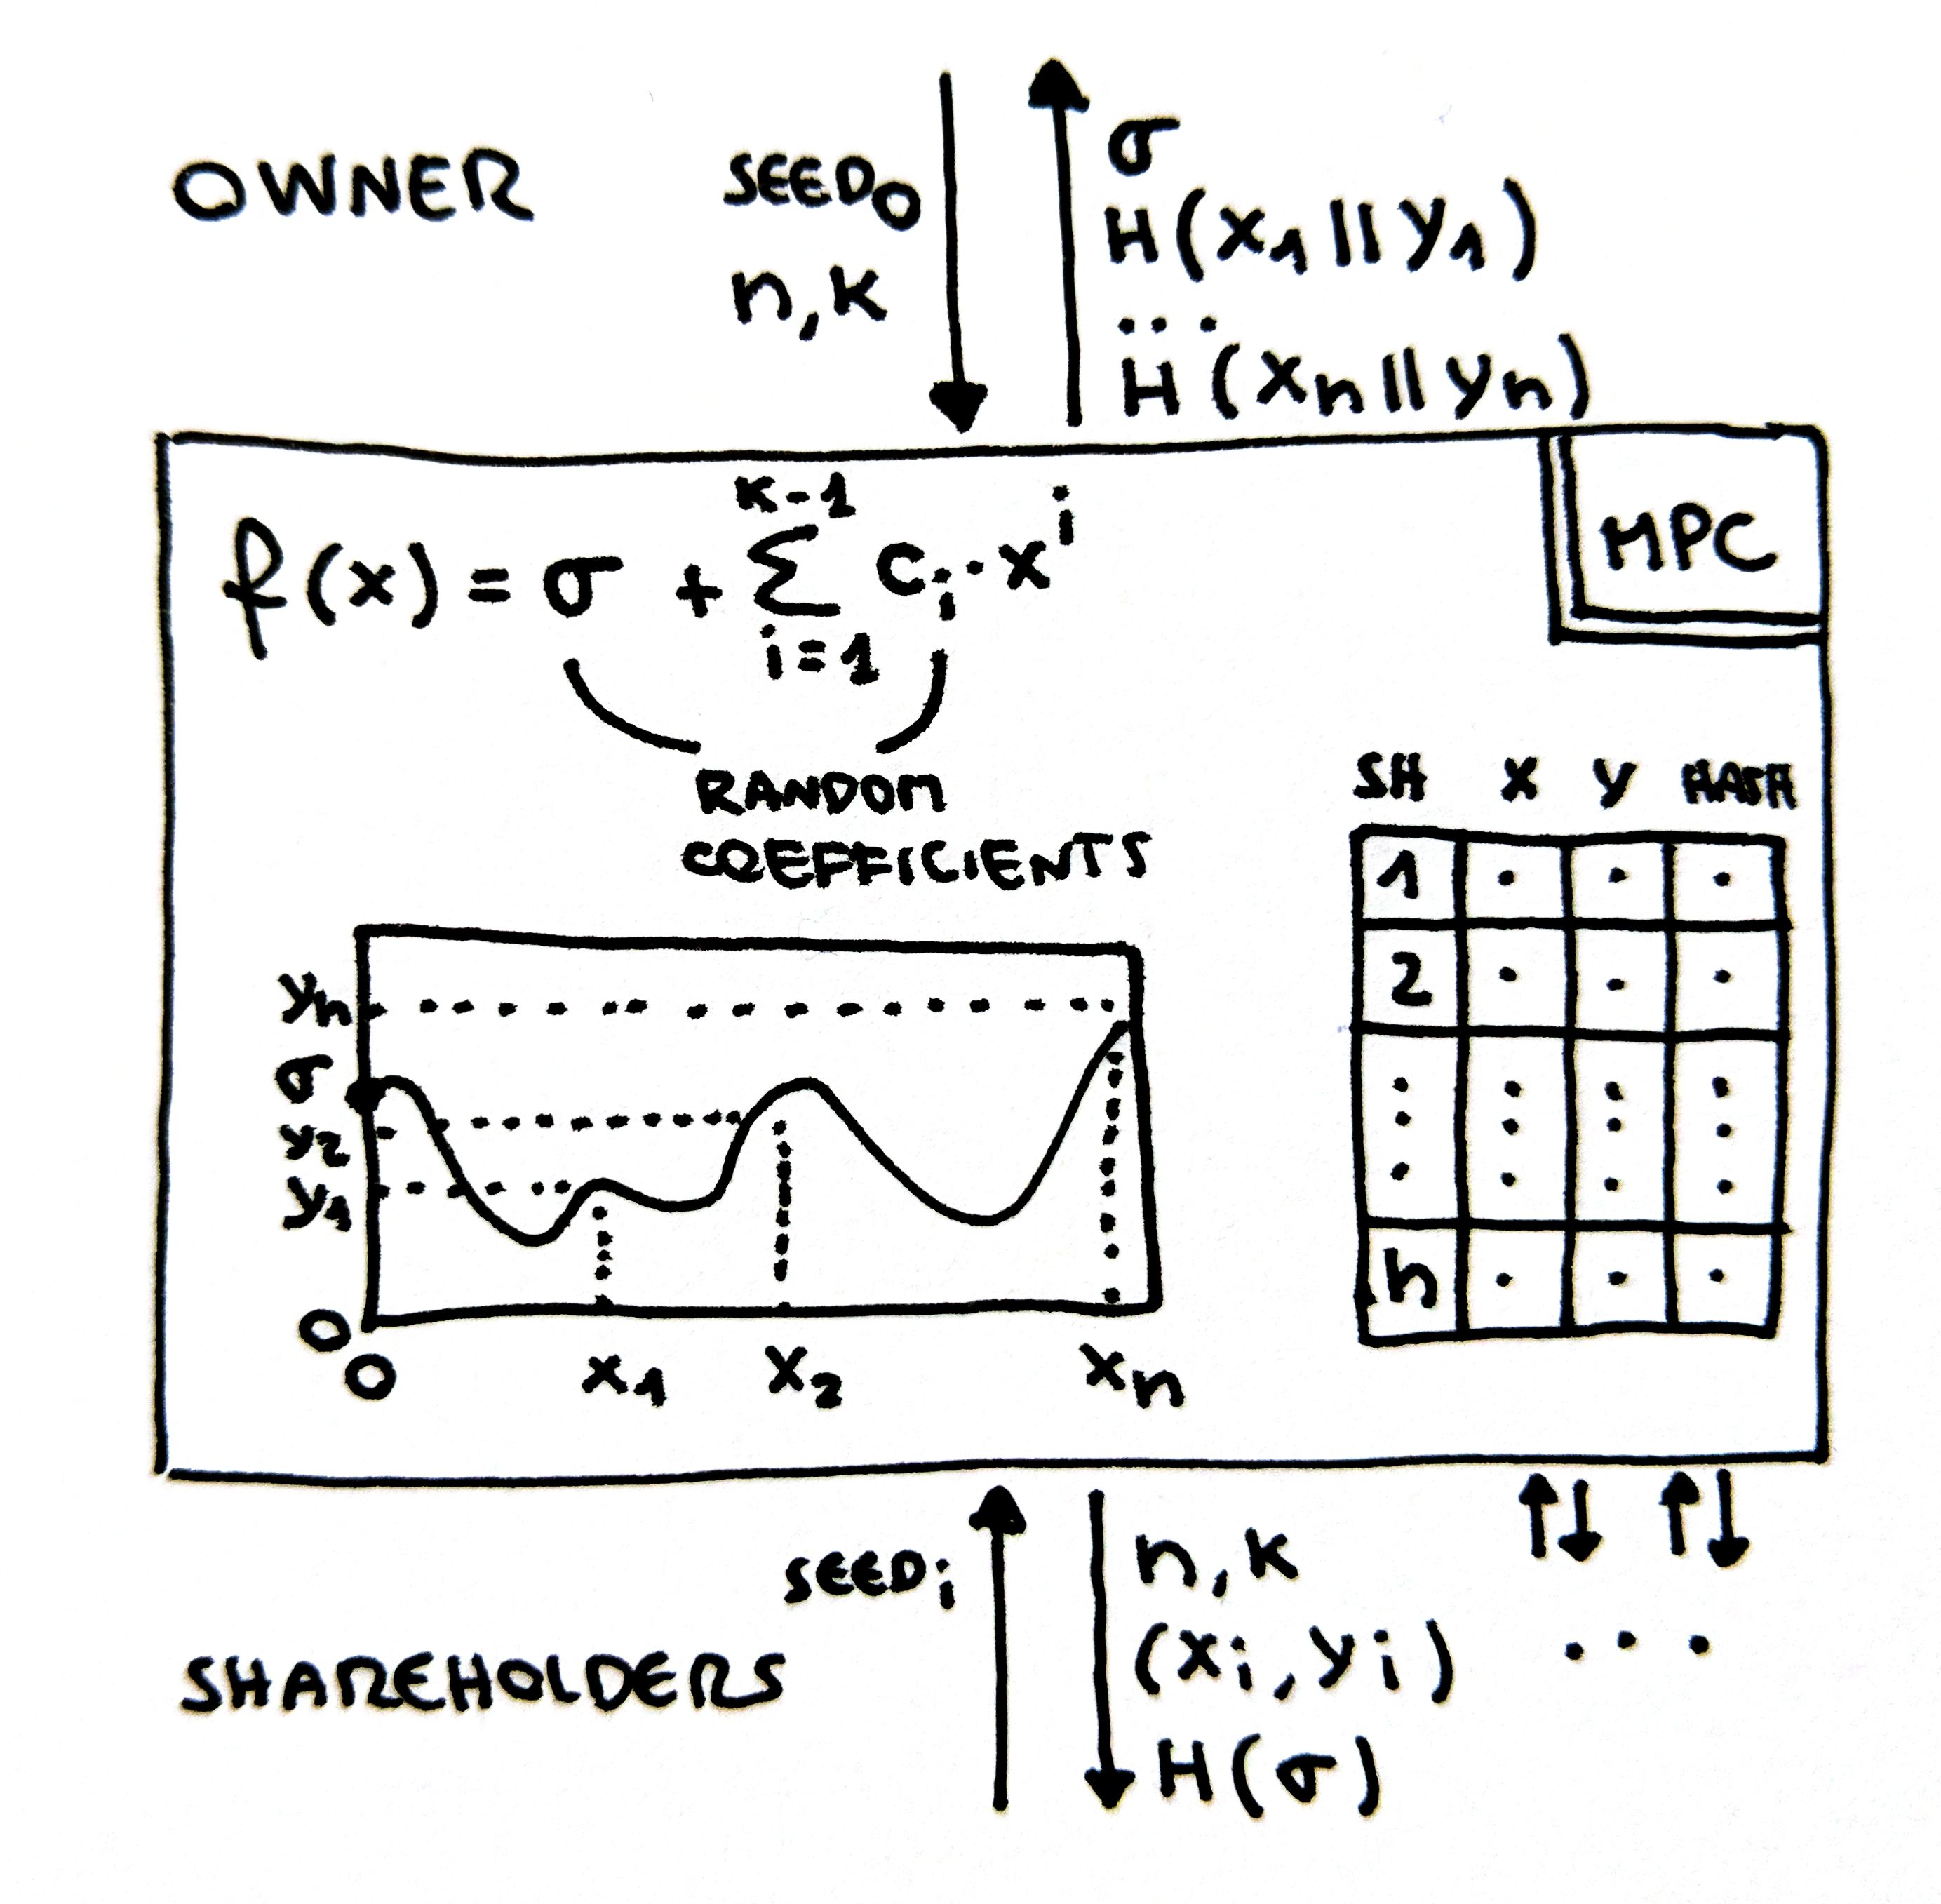
\includegraphics[width=.45\textwidth]{fig/mpc1} }} \\[20pt]
	\subfloat[Two Phases MPC Protocol]{{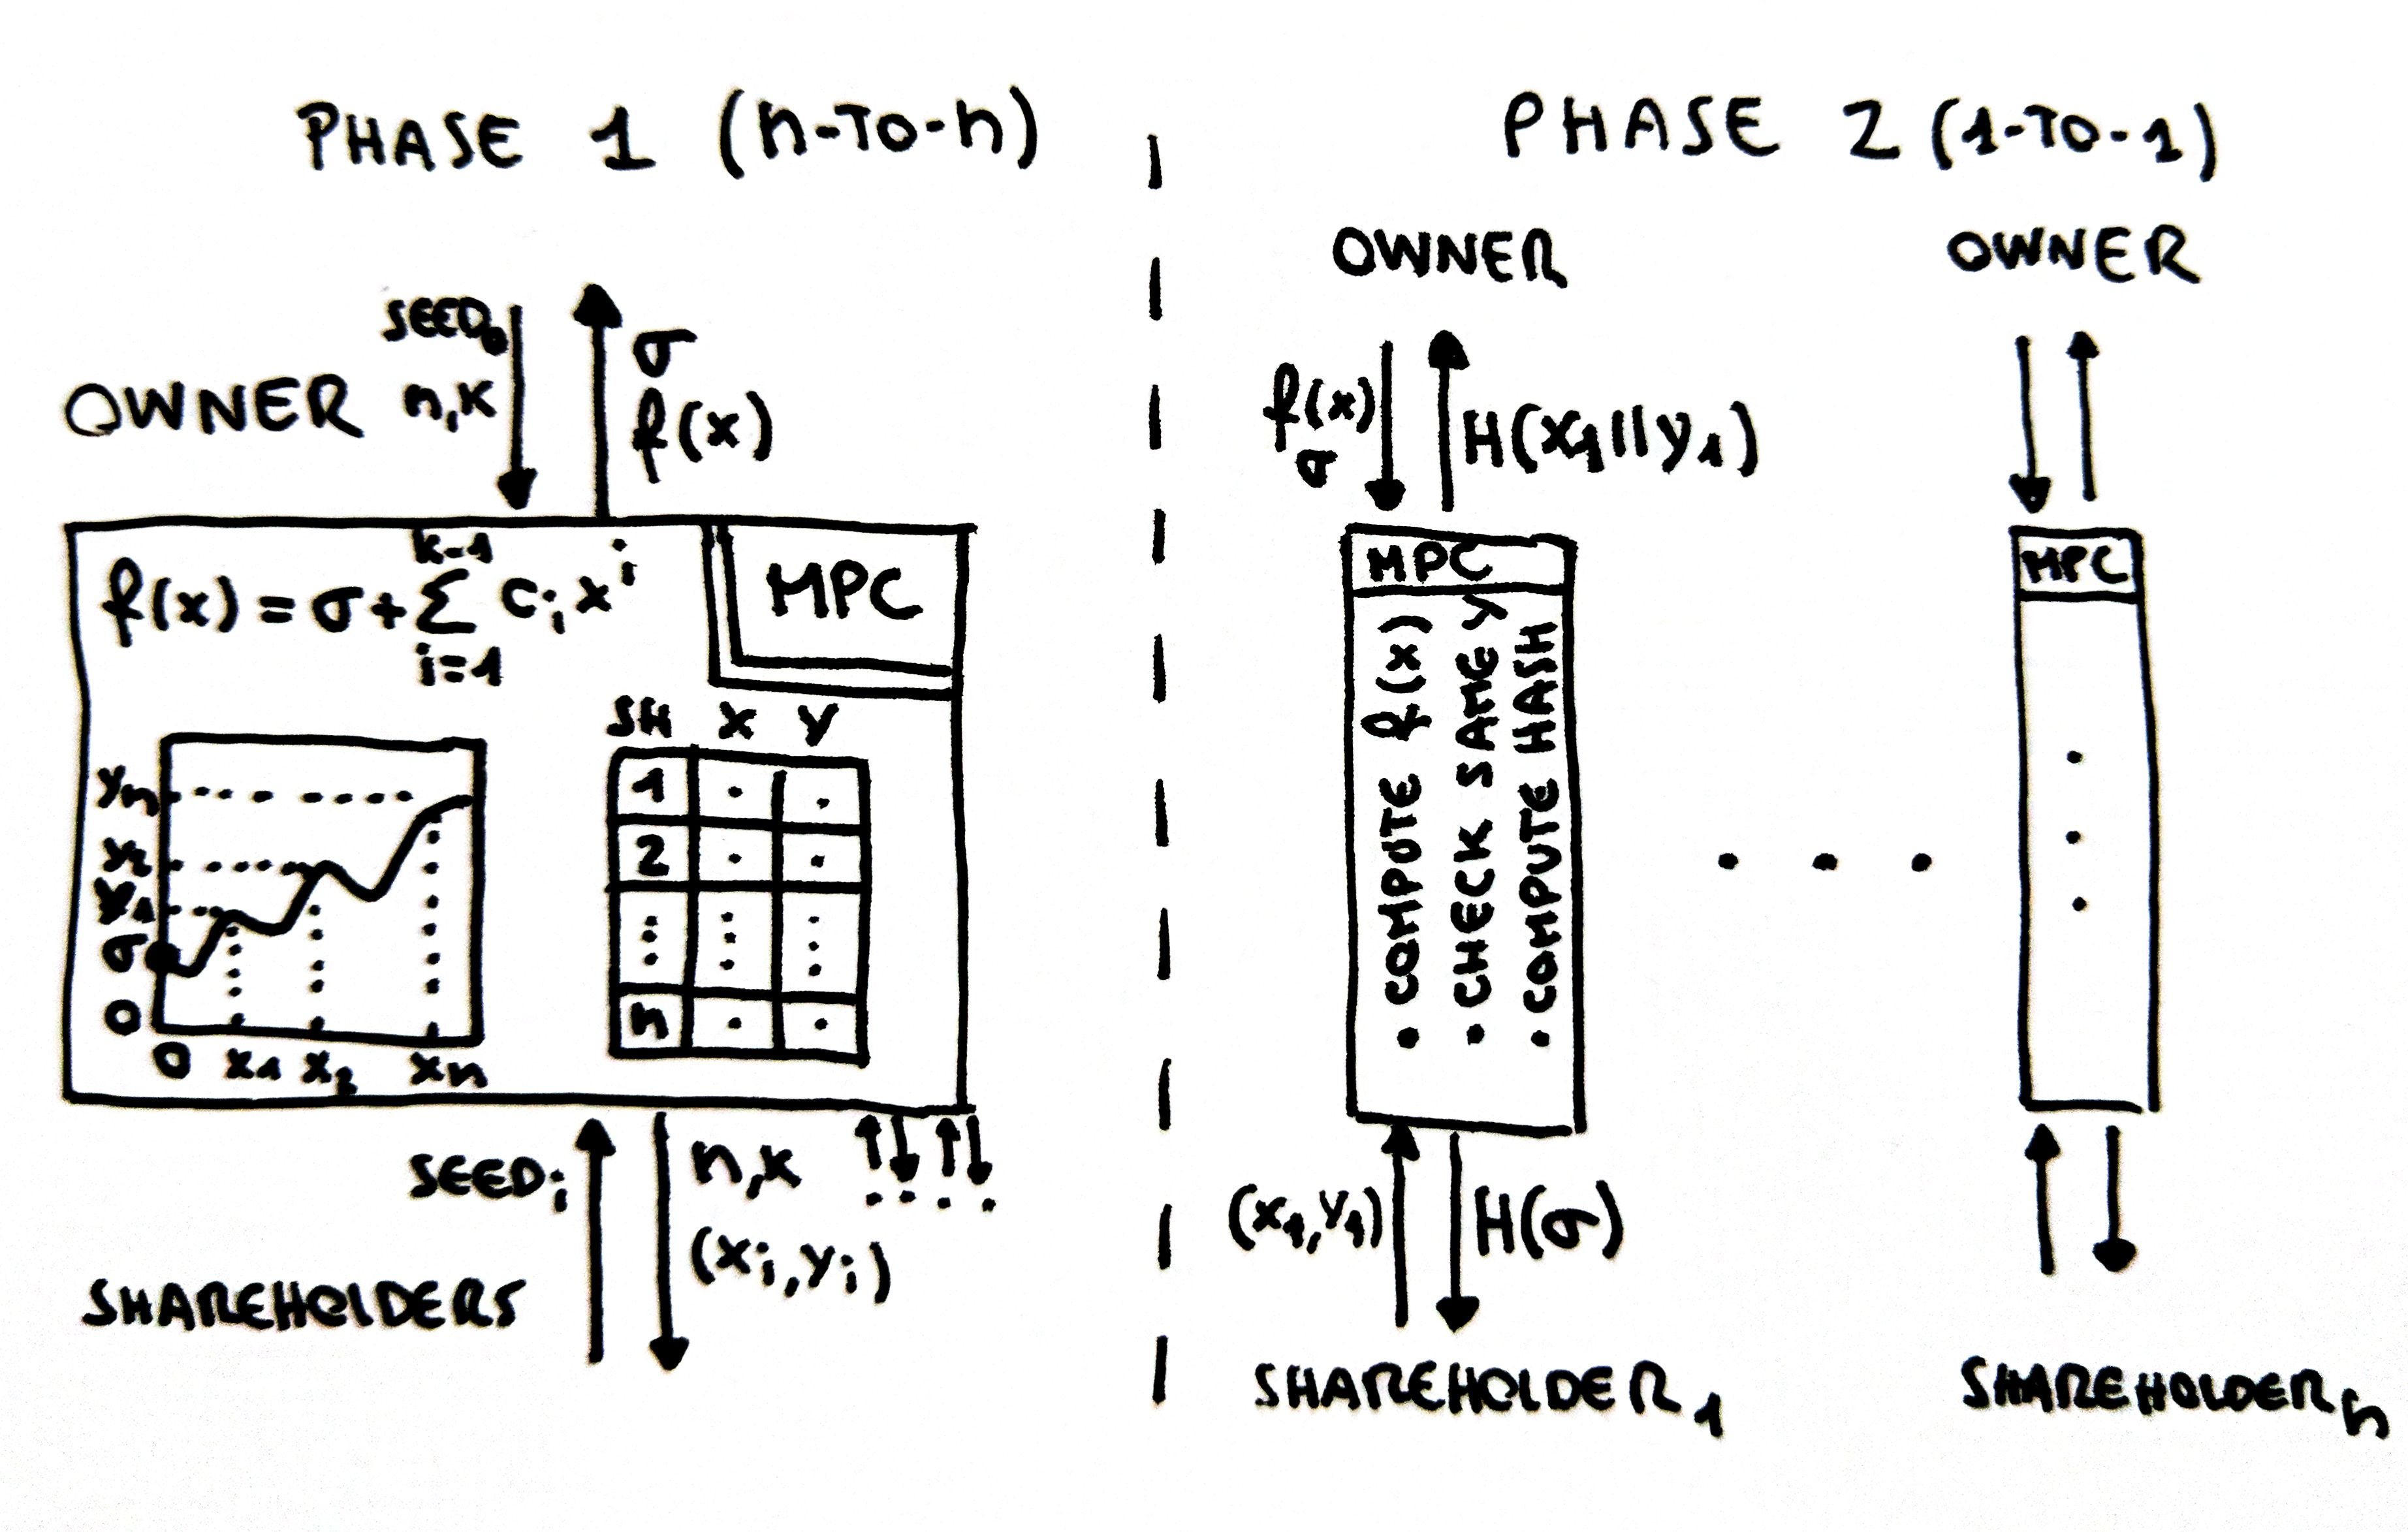
\includegraphics[width=.7\textwidth]{fig/mpc2} }} \\[20pt]
	\caption{Diagram description of the two kind of \shortname MPC protocols.}%
	\label{fig:mpc}%
\end{figure*}

This section illustrates how to practically implement the protocol described. 

As we anticipated in Sections~\ref{sect:introduction} and~\ref{sect:background}, the following three technologies are the pillars of our construction:
\begin{itemize}
	\item the blockchain, the technological layer which allows us to publicly store the history of the protocol and persistently disclose the secret;
	\item smart contracts, the mechanism that allows us to set economic incentives and penalitations in a fully decentralized execution environment without the need of a trusted third party;
	\item sMPC, the instrument through which it is possible to securely execute cryptographic operations between multiple hosts.   
\end{itemize}

Before start describing our approach, we briefly highlight some problems which have to be addressed in order to get the desired execution.
\newline
A smart contract cannot be corrupted or blackmailed, as it always act deterministically accordingly to the specified algorithmic procedures stored inside it, upon which the parties have agreed consent. 
However, in order to deploy one valid instance of a smart contract, one user has to send a transaction from his wallet to the blockchain. Since the deployment request has to be sent by one party to another one (i.e., the blockchain), and since such request can not be performed inside an MPC protocol, only one among the owner and the shareholders must be in charge of that.  
The selected user, typically the owner, could manipulate the validated data received as output from an MPC protocol before sending them to the smart contract. As an example, the owner could change the commitments to prevent the shareholders to ever receive their rewards and therefore jeopardizing the whole protocol.
\newline
Another problem is that, although the blockchain permits the decisions taken by the participants of the protocol to be fully transparent to the whole network, it is not immediate how to manage internal coordination. Unlike what happens in common situations, before being able to proceed with some actions, it is necessary to reach the consensus among all the participants and not only among the majority of them. As an example the owner might desire all the shareholders to deposit their bids before to start distributing the shares.
All such erroneous situations and illegal modifications have therefore to be prevented.

\subsection{Our approach}\label{sect:our_approach}

\paragraph{Short description} 
In order to solve the issues described, we designed \shortname protocol as a state machine implemented inside an Ethereum smart contract. The state of the protocol can be evolved by performing some actions, each action maps to a specific smart contract function, and when executed, each function produces a transaction that is spread across the whole blockchain and is validated by all its nodes. Furthermore, before participating to a specific instance, each candidate can verify the algorithmic code contained inside the contract. 
\newline
A simplified version of the state machine describing the protocol (see Figure~\ref{fig:fsm}) is characterized by two phases: a \texttt{setup phase}, in which the owner and the shareholders have to cooperate in order to deploy, configure and activate one instance of the protocol, and an \texttt{enforcing phase}, in which the participants comply with the constraints of the contract and thus effectively implementing the time lock primitive.

\medskip\textbf{Phases of execution.} The following description illustrates each of the two execution phases in detail.


\paragraph{Setup phase - I}
Initially, the owner deploys an instance of \shortname on the Ethereum blockchain. 
By calling the function \texttt{configure}, she sends to the contract the pawn, $\PO$, and she is then able to specify all the information about participants, the economic conditions and the time thresholds required for the correct execution, thus landing the protocol to the state \texttt{pre initialized}. 
To demonstrate the will to correctly participate, each shareholder calls \texttt{deposit} and transfers to the contract the proper amount of Ether corresponding to the bid, $B_{\mathcal{H}}$. 
The owner observes the actions taken by all the participants by reading the state of the contract, and, after she notices all the shareholders have asserted on the continuation, she then writes on the blockchain the state \texttt{initialized} by calling the function \texttt{startMPC}. The latter action permits to open the sMPC time window, during this time interval all the participants cooperate in order to bring to completion the secure multi-party computation protocol. The entire execution of the sMPC protocol takes place outside the blockchain, specifically, in the form of a network computation protocol.

\paragraph{sMPC protocol}\label{sect:impl_mpc_brief}
We use the sMPC protocol as a tamper proof primitive which permits to securely generate a random key, $\key$, and a set of $n$ of its shares $\left\lbrace \share _0 , \ldots , \share_{n-1} 	\right\rbrace$. Specifically, the shares are derived from the key using the Shamir's Secret Sharing algorithm~\cite{Shamir:1979:SS:359168.359176}, so that it is possible to reconsruct $\key$ out of {\em k-of-n} shares.
$\key$ is primarily necessary for two reasons: first, it will be used by $\owner$ to wrap the $\secret$ by an encryption algorithm $\cipvocabulary$, and second, it permits to avoid the exposition of $\secret$ until the current \shortname instance has been activated.  
\newline
In order to execute the sMPC protocol the owner has to input the total number of shareholders, $n$, together with the reconstruction threshold, $k$. Each shareholder is instead relieved from the input of any date. Along with the input, each participant, be it the owner or a shareholder, can opt for the insertion of a random seed, this can be done to increase the entropy, and therefore the security, of the protocol. As output of the sMPC protocol, $\owner$ receives $\key$ and a commitment $\commitment _i$ of any share generated\footnote{With commitment share we denote the hash of the share.}, while each shareholder receives her share $\share_{i}$, a commitment of the key $ \commitment _ \key $, $n$ and $k$. 
A representation of the sMPC described can be seen in Figure~\ref{fig:mpc}a. 
\newline
Before to continue describing the {\em setup phase}, we briefly remind that the sMPC permits to keep the input and output of each participant private, this as an example, guarantees each shareholder that no one, except herself, will be able to submit her share at disclosure time. The use of an sMPC is then fundamental to guarantee the economic game conditions over which our analysis is based. Further important implications about the use of an sMPC will be discussed later, in Subsection~\ref{sect:impl_mpc}.

\paragraph{Setup phase - II}
Once the sMPC has terminated, all the participants have the information required in order to correctly run the protocol, hence, all that remains to do is to conclude the smart contract configuration and proceed with \shortname activation. In order to accomplish that, the owner calls the function \texttt{finalizeMPC} and sends to the contract the commitment of the key, $ \commitment _\key $, along with the commitments of all shares, $\{ \commitment _i , ... , \commitment _n \}$. The last action changes the state to \texttt{pre committed} and permits to close the sMPC window. Each shareholder can then read the data written by $\owner$ and verify their correctness, in particular, if the information corresponds to the one output from the sMPC, each shareholder will perform a \texttt{commit}. After each of them has committed, the owner calls \texttt{enforce} and therefore activates the current instance of \shortname (i.e., activation of all the penalties against adversaries) landing the state to \texttt{LOCK} and concluding the {\em setup phase}. 

\paragraph{Enforcing phase}
Once the TL is active, before going offline, the owner can opt for both:
\begin{itemize}
	\item[1.] using the key to wrap the secret (from now on we will use plaintext, \plaintext, as synonym for secret) with the selected encryption algorithm in order to produce the ciphertext, \ciphertext $=$ \wrap;
	\item[2.] permanently writing \ciphertext on the Blockchain by calling the function \texttt{loadSecret}.
\end{itemize}
The reason why the execution of the aforementioned steps is optional is that the actual configuration of the protocol is totally agnostic to the presence of \ciphertext or to the meaning of \secret, this because the outcome of \shortname is only bounded to the disclosure of the key. 
In fact, the possession of \key demonstrates one among: its mismanagement by the owner or the collusion among the shareholders; it is impossible to discriminate between them.   
Anyone in possession of a $\key \sp{\prime} $ can therefore proceed with its submission by performing the whistleblow action. 
Before  triggering all the penalties to the participants and transferring the whistleblower bonus, \Wbonus, to the sender, the code of the \texttt{whistleblow} function checks for the equality between  $\commitment _ { \key \sp{\prime} } $ and $\commitment _ \key $. 
If that was the case, the protocol would reach the final state \texttt{FAIL} and consequently all the money locked by the contract would be burned.
Alternatively, if no adversarial coalition will reconstructs \key before the disclosure time \td, then anyone can call the function \texttt{conclude} to terminate the protocol (\texttt{UNLOCK} state) and give all the shareholders the possibility to earn the reward by permanently write their shares to the blockchain. The function that permits to deposit a share is \texttt{registerShare}, each reward is payed if and only if the share is considered valid (i.e., it satisfies its correspondent commitment).
\newline
Finally, we highlight that we do not need an implementation of the secret reconstruction functionality, this because:
\begin{itemize}
	\item the blockchain will permanently and publicly store all the valid shares; 
	\item anyone interested in the secret will extract the \key and then recover the plaintext loaded by the owner by performing \plaintext $=$ \unwrap.
\end{itemize} 



\begin{figure}[t]
	\centering
	\subfloat[A colluding coalition could reveal \secret before paying the bids] {{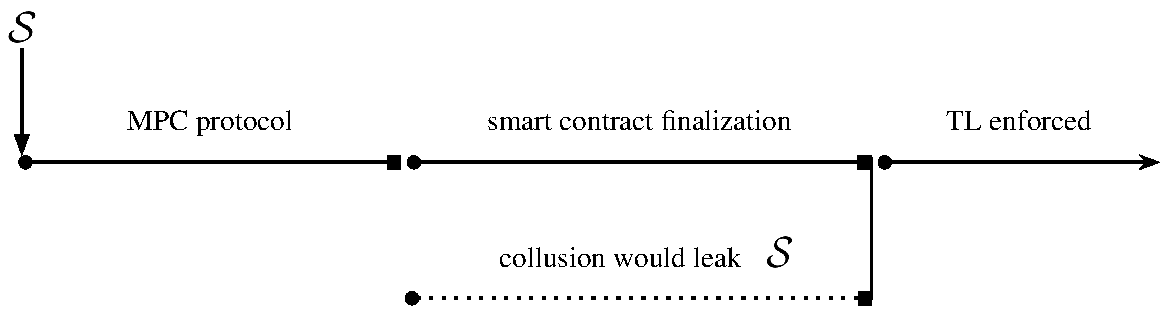
\includegraphics[width=0.7\columnwidth]{fig/time1} }}\\
	\subfloat[A colluding coalition could only reveal $\sigma$ before paying the bids] {{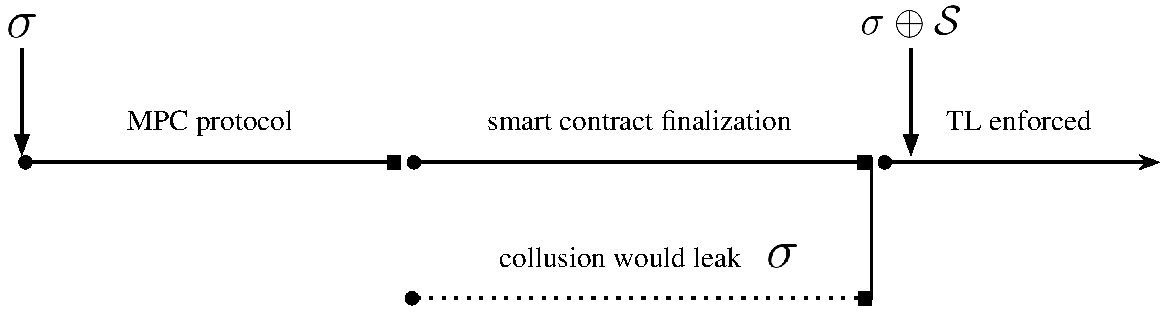
\includegraphics[width=0.7\columnwidth]{fig/time2} }}
	\caption{Time diagram for the generation of the secret}%
	\label{fig:sigmatime}%
\end{figure}


\subsection{Safe usage of sMPC protocols}\label{sect:impl_mpc}


The discussion so far has focused on the single user perspective regarding the sMPC protocol, namely its role was seen primarily as a defensive one. The shareholder $\shareholder_{i}$ is in fact guaranteed that no other user, including the owner, will have visibility on the $i$-th share, $\share_{i}$. The latter and further capabilities are fundamental in order to limit the knowledge of each single user about each instance of the TL protocol, making it possible to model it as an economic game. 

Anyway, if we take the perspective of a group of users and not of an individual, the role of sMPC protocols reverses. The malicious coalition of shareholders, \coalition, could devise a strategy that permits the reconstruction of \secret without incurring economic penalties. 
Such a strategy is successful if makes impossible for anyone to carry out the whistleblow action. By referring to the notation introduced in~\ref{sect:our_approach}, we say that a strategy is successful if it permits to reconstruct the \plaintext without exposing the \key. 
As a matter of fact, the malicious coalition can successfully attack the protocol by instantiating an offensive sMPC that receives as input at least $k$-of-$n$ shares and the ciphertext, \ciphertext, and internally performs both the SSS reconstruction of \key and the extraction \unwrap of \plaintext, sending to all the participants the latter as the only output. 

In order to prevent \coalition executing a successful attack it is required to select a cryptosystem \cipvocabulary such that there is no sMPC protocol that can permit to execute \dec by producing \plaintext as the only output. There are two possible alternatives to satisfy the previous requirement: the first one is to select cryptosystems whom execution is not compatible with sMPC protocols, while the second one is to ensure that the exposition of \plaintext implies the one of \key.
It easy to satisfy the second alternative, indeed, by selecting $\cip = \onetimepad$ is it easy to prove that given two among $\{ \ciphertext , \plaintext , \key \}$ the third is implied. Thus, each member of a malicious coalition would turn to a potential whistleblower after the execution of the adversarial sMPC.

--
\newline
DA QUI IN POI ANCORA DA RISTRUTTURARE

\subsection{Additional smart contract features}

Within the smart contract we have also implemented other functionalities to prevent deadlocks and other malfunctions.

\begin{figure*}[t]
	\centering
	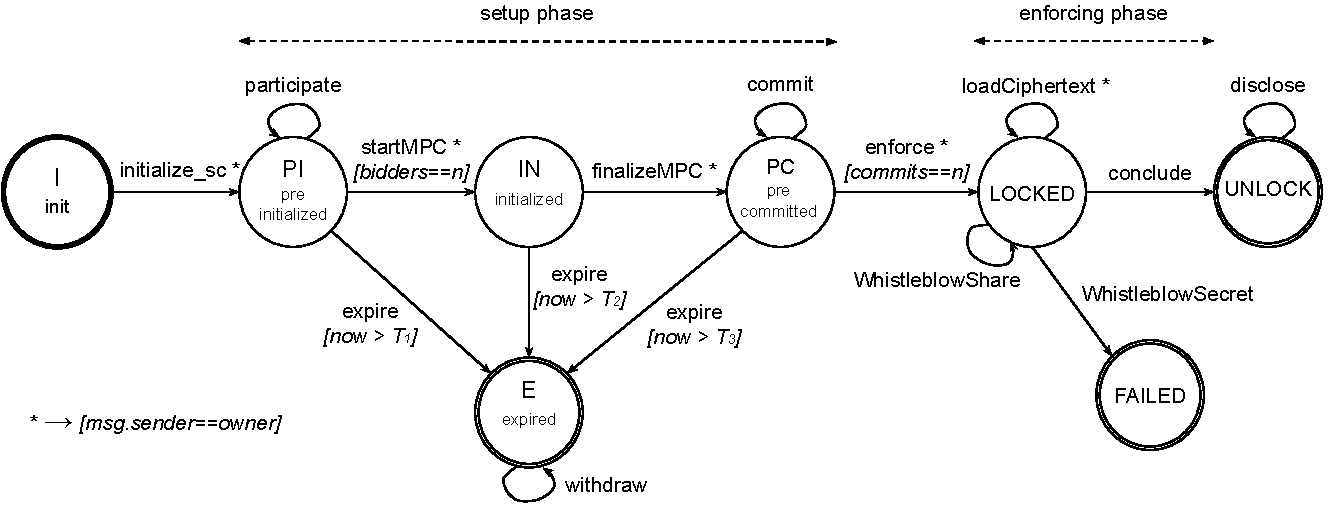
\includegraphics[width=\textwidth]{fig/protocol_fsm_simple_version}
	\caption{State machine representing the evolution of \shortname protocol. Each transition name maps to an action (an Ethereum smart contract function) each participant of the protocol can to perform in order to modify its state. Square brackets contain additional conditions to be met in order to make each transition valid.}
	\label{fig:fsm}
\end{figure*}
 
\paragraph{Facilitating disclosure}

In order to met the additional constraints introduced in subsection~\ref{subsect:fac_discl}, we allowed the owner to set a maximum disclosure time deadline, or rather the time instant to which the registration of less than $k$ shares determines the failure of the protocol. Furthermore we integrated the extra remuneration of $\delta$ for the fastest $k$ registering shareholders. 

\paragraph{Minimize DOS Attacks}

Since all the users have to submit a pawn or a bid for the contract to become \texttt{initialized}, a small fraction of users could perform a denial of service attack by taking part in many \shortname protocols refusing to deposit bids, commit or to correctly execute the sMPC. There are two ways to prevent these kind of disruptions. The first is to introduce a reputation system, so that the owner can select parties that are willing to co-operate. Obviously this would be an ideal choice that could benefit also other parts of our model. However, since a reputation model is not always possible to introduce, another option is to include in the smart contract model the {\em pre-considered} phase, in which all the participants (including the owner) are required to pay a small service pawn that will be returned only if the smart contract will reach the \texttt{LOCK} state. It has been proved that introducing a small fee to access a service can prevent many DOS attacks~\cite{ddos-payments,ddos-survey}. Anyhow, to keep the discussion as clear as possible, we decided to only include the presence of the additional final state \texttt{expired}, which permits each participant to withdraw the money locked by the contract itself, in case the activation time thresholds set by the owner were not met.  

\begin{comment}
It is possible to access the current block time using 'block.timestamp' ('now' is a synonym of this). The time will be returned as a POSIX timestamp (basically the monotonous number of seconds since 1970-01-01 00:00:00 UTC). However, this timestamp is 'set' by the miner that ends up mining your transaction. As such, the miner can manipulate the timestamp. There are certain rules to this; other parties will not accept a block if the given timestamp occurs in the future, for instance (more detail about this). But this does mean that the number cannot be used for e.g. random number generation.
\end{comment}


\begin{comment}
\begin{figure}[tp]
\centering
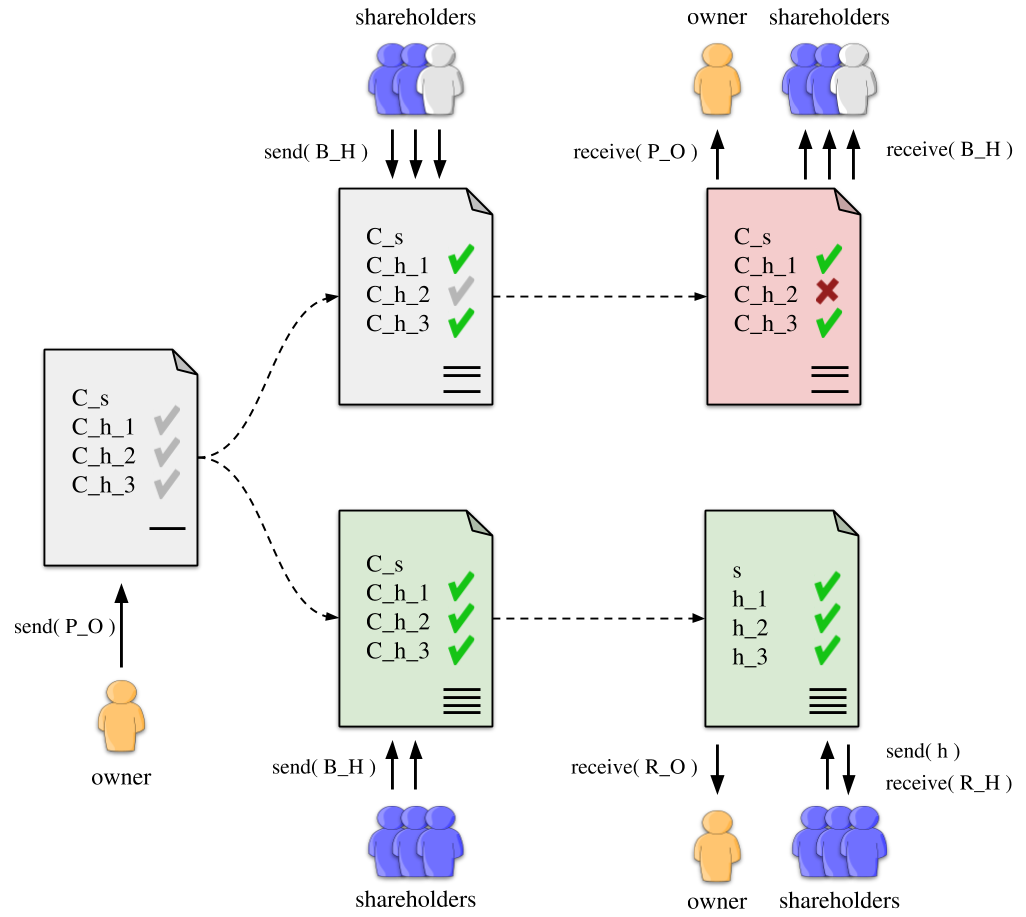
\includegraphics[width=\columnwidth]{fig/mssc}
\caption{Smart contract stages}
\label{fig:mssc}
\end{figure}
\end{comment}
